\documentclass[sigconf]{acmart}

\usepackage[english]{babel}
\usepackage{blindtext}
\usepackage{listings}

%\usepackage[compact]{titlesec}
\newcommand{\newtodo}[1]{\textcolor{red}{#1}}


\usepackage{enumitem}
\setitemize{noitemsep,topsep=0pt,parsep=0pt,partopsep=0pt}
\setenumerate{noitemsep,topsep=0pt,parsep=0pt,partopsep=0pt}
\setdescription{itemsep=0pt,topsep=0pt,parsep=0pt,partopsep=0pt,itemindent=0em,leftmargin=0.5em}

% \us: "microseconds"
\newcommand{\us}{\textmu{}s\xspace}

%compressed environments
\newenvironment{denseitemize}{
\begin{itemize}[topsep=2pt, partopsep=0pt, leftmargin=1.5em]
  \setlength{\itemsep}{2pt}
  \setlength{\parskip}{0pt}
  \setlength{\parsep}{0pt}
}{\end{itemize}}

\newenvironment{denseenum}{
\begin{enumerate}[topsep=2pt, partopsep=0pt, leftmargin=1.5em]
  \setlength{\itemsep}{2pt}
  \setlength{\parskip}{0pt}
  \setlength{\parsep}{0pt}
}{\end{enumerate}}

\def\ie{{i.e.\ }}
\def\eg{{e.g.,\ }}
\def\etal{{et al.\xspace}}
\def\wrt{{w.r.t.\xspace}}
\def\etc{etc.\xspace}

\def\name{\texttt{cache\_ext}\xspace}

\newcommand{\tailpct}[0]{99\textsuperscript{th}-percentile}
\newcommand{\tailpctnnn}[0]{99.9\textsuperscript{th}-percentile}

\newcommand{\taillatency}[0]{\tailpct{} latency}
\newcommand{\taillatencynnn}[0]{\tailpctnnn{} latency}

\iftrue
\newcommand{\asaf}[1]{\textcolor{red}{\{Asaf: #1\}}}
\newcommand{\tal}[1]{\textcolor{red}{\{Tal: #1\}}}
\newcommand{\teng}[1]{\textcolor{red}{\{Teng: #1\}}}
\else
\newcommand{\asaf}[1]{}
\newcommand{\tal}[1]{}
\newcommand{\teng}[1]{}
\fi

\newcommand{\uffd}{\texttt{userfaultfd()}}

% Copyright
\renewcommand\footnotetextcopyrightpermission[1]{} % removes footnote with conference info
\setcopyright{none}
%\setcopyright{acmcopyright}
%\setcopyright{acmlicensed}
%\setcopyright{rightsretained}
%\setcopyright{usgov}
%\setcopyright{usgovmixed}
%\setcopyright{cagov}
%\setcopyright{cagovmixed}

\settopmatter{printacmref=false, printccs=false, printfolios=true}

% DOI
\acmDOI{}

% ISBN
\acmISBN{}

%Conference
%\acmConference[Submitted for review to SIGCOMM]{}
%\acmYear{2018}
%\copyrightyear{}

%% {} with no args suppresses printing of the price
\acmPrice{}


\begin{document}
\title{Custom Page Fault Handling With eBPF}

\author{Paper \# XXX, XXX pages}

% The default list of authors is too long for headers}
\renewcommand{\shortauthors}{X.et al.}

\begin{abstract}
Traditionally, page faults have been handled by the OS kernel, with a fixed set of handling routines for different types of faults. However, some applications may benefit from custom page fault handling routines, allowing them to implement advanced functionality. To this end, the \texttt{userfaultfd()} syscall, which allows applications to handle their page faults in userspace, was introduced on Linux. While \texttt{userfaultfd()} has proven useful in a number of applications, we identify some key deficiencies in its design which limit both performance and applicability. We propose a system which allows using eBPF programs to handle page faults in-kernel, reducing context switching and enabling novel use cases.
\end{abstract}



\maketitle



\section{Introduction}
\label{sec:introduction}

%===================Background=====================%

% While it is conventional for the operating system kernel to handle page faults, delegating page fault handling to the userspace has proven to be more flexible in some use cases (in some impactful projects.)

While it is conventional for the operating system kernel to handle page faults, certain prevalent open-source projects have demonstrated the flexibility gained by delegating page fault handling to the userspace.

In Linux, the \textt{userfaultfd()} system call implements such functionality. It is "a proper and more optimal implementation of the PROT\_NONE+SIGSEGV trick.", according to xxx (\teng{How to put this?})
% This page is good. summarize with it: https://docs.kernel.org/admin-guide/mm/userfaultfd.html

%===================uffd mechanism breakdown=====================%
The story of \textt{userfaultfd()} is 
1 faulting thread and one fault handling thread.

domain socket

epoll

userfaultfd was originally developed for container and virtual machine migration.

Live migration can be crucial for large cloud providers, for example, to move client virtual machines out of a failing node transparently. According to Google, live migration is commonly used for VM/Host software Upgrades, Load Balancing, and so on\cite{google-live-migration-at-scale}.

Specfically, post-copy xxx\cite{post-copy}



https://lore.kernel.org/kvm/20230412213510.1220557-1-amoorthy@google.com/T/

%===================Use Cases=====================%

https://tech.nextroll.com/blog/data/2016/11/29/traildb-mmap-s3.html
%===================Use Cases=====================%
CRIU, a xxx, is using userfaultfd()

Firecracker, a xxx, also supports using uffd to let an external process to handle its guest memory page fault

% Firecracker then sends the memory ranges descriptions/mappings along with the Uffd over a UnixDomainSocket specified in 'backend_path' parameter on the API call.

% We need one sentence to show how performance of post-copy migration, for example:

Pre-copy copies states including memory. Post-copy copies states except memory.


https://ieeexplore.ieee.org/stamp/stamp.jsp?tp=&arnumber=9786612
Copying 16GB memory data takes more than 6 minutes in
pre-copy migration. On the contrary, the downtime of post copy migration is only about 320 ms


https://kartikgopalan.github.io/publications/hines09postcopy_osr.pdf
https://duasynt.com/blog/cve-2016-6187-heap-off-by-one-exploit


QEMU/KVM uses the \texttt{userfaultfd()} system call to implement \textit{postcopy live migration}


Migration is not the only use case of \uffd. It's been gathering attention for the flexibility it provides. UMap\cite{file-backed-article, file-backed-proceeding} is a project 


%===================Our Work=====================%

In this extended abstract, we leverage eBPF infrastructure to delegate page fault handling to eBPF programs, which potentially provides a performant and secure way for applications to customize page fault handling.



In the motivation part, we will conduct experiment on the userfaultfd to expose its performance and security issues.



Userfaultfd exposes safety issues 
\section{Motivation}
\label{sec:motivation}

\texttt{userfaultfd()}




\textbf{Latency/Performance issue}. 

\begin{itemize}
    \item Context switching and kernel-user copying (It does \texttt{copy\_from\_user()} when we do \texttt{ioctl()} with flag \texttt{UFFDIO\_COPY}, which is the most common way of handling for fault handling thread                                                                                                                                                ). (Not kernel crossing). We probably need a graph to illustrate this with the copying
    \item Polling. \uffd's fault handling thread pollings from the (\teng{or on}) the file descriptor. And incurs overhead. While you might alleviate the polling overhead with \texttt{epoll()}
\end{itemize}

\textbf{Resource utilization issue}
\teng{I don't know how to talk about this part. }


\textbf{Scalability issue}. Because \texttt{userfaultfd()} handlers Here we insert \ref{fig:motivation-scalability}


% \begin{figure}[tp]
% \centering
% \includegraphics{figures/mouse}
% \caption{This does not look good enough, might need to redraw it.}
% \end{figure}

\begin{figure}
        \centering
        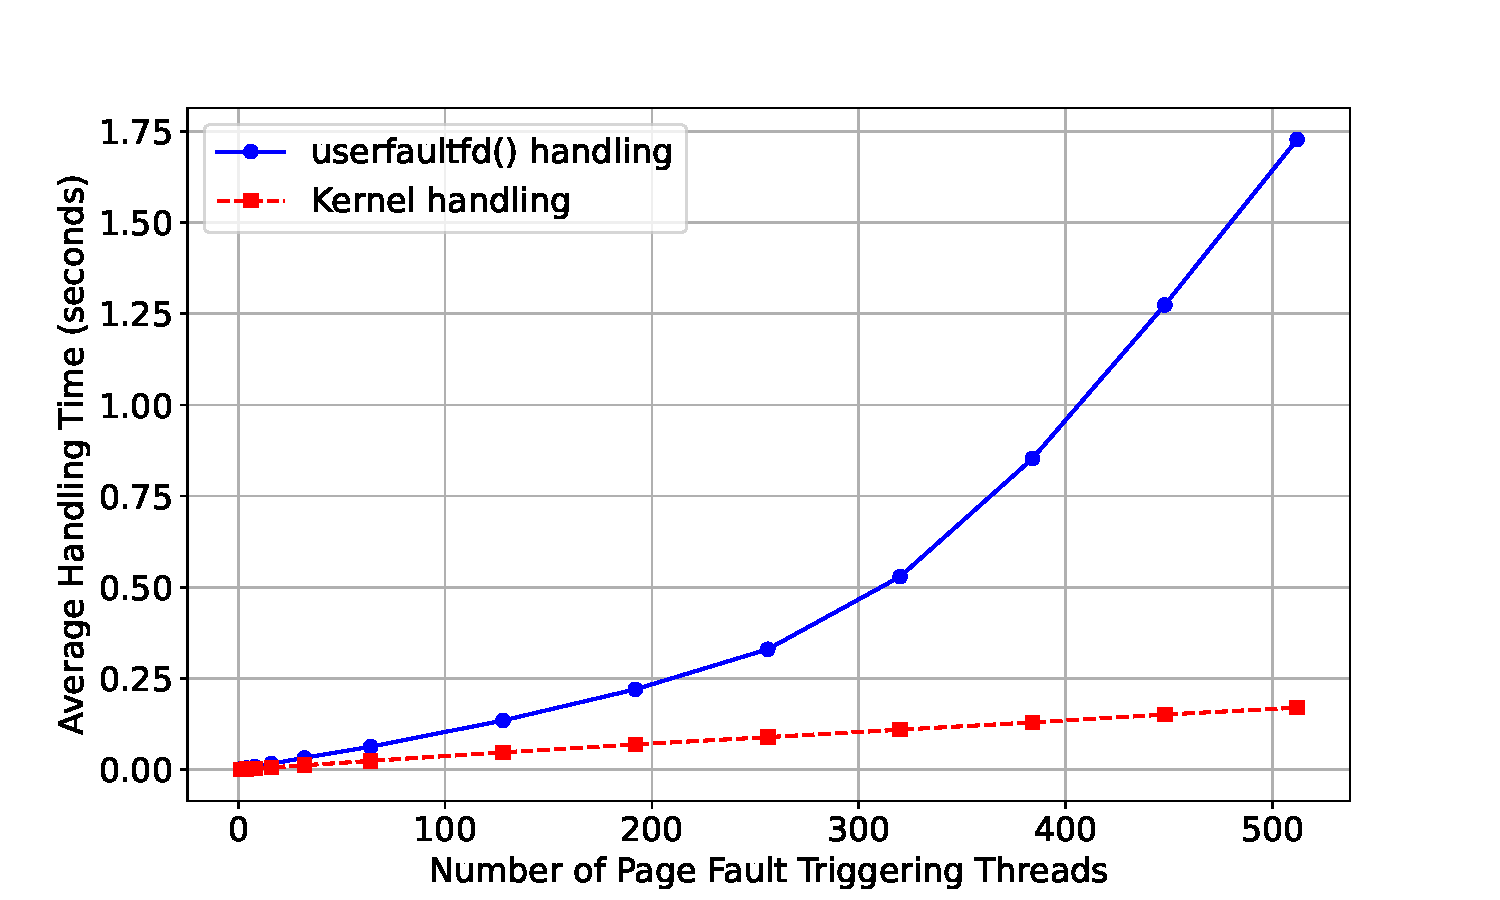
\includegraphics[clip,scale=0.33]{figures/motivation_scalability.pdf}
        \caption{To be added.}
        \label{fig:motivation-scalability} 
\end{figure}



% It does \texttt{copy\_from\_user}

\textbf{Security issue} \uffd might block the kernel\cite{uffd-blocking}, and is a common technique for kernel exploitation. For example, if the page fault handler choose to sleep (and nothing prevents it from doing that), the faulting thread will be stuck. This makes it easier to manipulate the execution order of process, and can be used to trigger race conditions on purpose. \teng{My point is, probably ebpf verifier can check for this?}

% No, eBPF programs cannot actively sleep like userspace programs can. However, they can call helper functions that can sleep, such as bpf_copy_from_user_stack. For example, a sleepable BPF program can call the bpf_copy_from_user_task helper when helper execution may be interrupted. However, the program doesn't have control over how long the helper function will sleep. 

Also, heap spraying (can ebpf solve this?)
https://etenal.me/archives/1336
\section{System Design}
\label{sec:design}


 Figure xxx is the overall design of our eBPF-powered page fault-handling routine.

 

 % \textbf{Initialization}. We first communicate with the BPF-fault subsystem to learn about what features are available (This is  UFFDIO_API but I guess we don't need it.)

\textbf{Loading}. When loading the eBPF program, the user specifies how page faults should be handled. \teng{Where should we discuss how to resolve page faults (the scratch memory design?)}
% There are three basic ways to resolve user faults:

% UFFDIO_COPY atomically copies some existing page contents from userspace.

% UFFDIO_ZEROPAGE atomically zeros the new page.

% UFFDIO_CONTINUE maps an existing, previously-populated page.

\textbf{The eBPF verifier} will be able to do checking in multiple folds (general, like dereferencing NULL pointer, and application-specific, like type of the fault handling, ... Refer to uffd)

\textbf{Attaching} the eBPF program to the \texttt{vm\_area\_struct}. When attaching the program, we need to split/merge virtual memory areas correspondingly.


When a page fault occurs, we "intercept" the page fault and call \texttt{handle\_bpf\_fault()} instead of going further into xxx. In a real application, the memory might be stored locally in persistent storage, or stored remotely - (We might be able to leverage XRP and XDP here?)

Notice that since eBPF programs run in the kernel, kernel crossing is bypassed.

\textbf{Runtime update \teng{I don't know what to call this}}. When memory space changed, the program reference count need to increment/decrement accordingly, and some policies need to be enforced. \texttt{mremap()}, \textt{munmap()}, \texttt{fork()}}. Which functionality need to be implemented largely depends on the use case.

 

This is the design.

We expect our eBPF solution will address the flaws of the \texttt{userfaultfd()} in the following ways:
\begin{itemize}
    \item $\uffd$ uses a fault handling
    \item $\uffd$ has a polling thread, while we handle page faults on the fly
    \item $\uffd$ incurs kernel crossing and memory copying, while we handle things purely in the kernel space.
    \item $\uffd$ has security issues, while ...
\end{itemize}



% \section{Evaluation}
\label{sec:evaluation}
Could be empty, depending on whether we put it in the motivation section or this section.
\section{Conclusion \& Research Agenda}
\label{sec:conclusion}

This is the conclusion. Plus Research agenda and/or Future Work.

In this paper, we have identified the space for improvements for \uffd. We proposed the 

ELF might be a good case to showcase what bpf-fault can achieve that $\uffd$  cannot.

\section{TODO}
\teng{header and footer}

The abstract is a little too vague.
\begin{lstlisting}
static inline bool vma_can_userfault(struct vm_area_struct *vma,
				     unsigned long vm_flags)
{
	if ((vm_flags & VM_UFFD_MINOR) &&
	    (!is_vm_hugetlb_page(vma) && !vma_is_shmem(vma)))
		return false;
#ifndef CONFIG_PTE_MARKER_UFFD_WP
	/*
	 * If user requested uffd-wp but not enabled pte markers for
	 * uffd-wp, then shmem & hugetlbfs are not supported but only
	 * anonymous.
	 */
	if ((vm_flags & VM_UFFD_WP) && !vma_is_anonymous(vma))
		return false;
#endif
	return vma_is_anonymous(vma) || is_vm_hugetlb_page(vma) ||
	    vma_is_shmem(vma);
}

\end{lstlisting}


\bibliographystyle{ACM-Reference-Format}
\bibliography{reference}

\end{document}